% Seminar 8: Extensii moderne
% Prezentare academică de calitate Harvard
% Program de licență, Academia de Studii Economice din București

\documentclass[9pt, aspectratio=169, t]{beamer}

% Asigură încadrarea conținutului pe diapozitive
\setbeamersize{text margin left=8mm, text margin right=8mm}

%=============================================================================
% CONFIGURARE TEMĂ ȘI STIL
%=============================================================================
\usetheme{default}

% Color Palette (matching Redispatch PDF)
\definecolor{MainBlue}{RGB}{26, 58, 110}
\definecolor{AccentBlue}{RGB}{26, 58, 110}
\definecolor{IDAred}{RGB}{205, 0, 0}
\definecolor{DarkGray}{RGB}{51, 51, 51}
\definecolor{MediumGray}{RGB}{128, 128, 128}
\definecolor{LightGray}{RGB}{248, 248, 248}
\definecolor{VeryLightGray}{RGB}{235, 235, 235}
\definecolor{KeynoteGray}{RGB}{218, 218, 218}
\definecolor{SectionGray}{RGB}{120, 120, 120}
\definecolor{FooterGray}{RGB}{100, 100, 100}
\definecolor{Crimson}{RGB}{220, 53, 69}
\definecolor{Forest}{RGB}{46, 125, 50}
\definecolor{Amber}{RGB}{181, 133, 63}
\definecolor{Orange}{RGB}{230, 126, 34}
\definecolor{Purple}{RGB}{142, 68, 173}

% Gradient background (exact Keynote 315 gradient: white to RGB 218,218,218)
\setbeamertemplate{background}{%
    \begin{tikzpicture}[remember picture, overlay]
        \shade[shading=axis, shading angle=315,
        top color=white, bottom color=KeynoteGray]
        (current page.south west) rectangle (current page.north east);
    \end{tikzpicture}%
}
% Fallback solid color for compatibility
\setbeamercolor{background canvas}{bg=}

\setbeamercolor{palette primary}{bg=MainBlue, fg=white}
\setbeamercolor{palette secondary}{bg=MainBlue!85, fg=white}
\setbeamercolor{palette tertiary}{bg=MainBlue!70, fg=white}
\setbeamercolor{structure}{fg=MainBlue}
\setbeamercolor{title}{fg=IDAred}
\setbeamercolor{frametitle}{fg=IDAred, bg=}
\setbeamercolor{block title}{bg=MainBlue, fg=white}
\setbeamercolor{block body}{bg=VeryLightGray, fg=DarkGray}
\setbeamercolor{block title alerted}{bg=Crimson, fg=white}
\setbeamercolor{block body alerted}{bg=Crimson!8, fg=DarkGray}
\setbeamercolor{block title example}{bg=Forest, fg=white}
\setbeamercolor{block body example}{bg=Forest!8, fg=DarkGray}
\setbeamercolor{item}{fg=MainBlue}

% Footer colors (override Madrid theme blue)
\setbeamercolor{author in head/foot}{fg=FooterGray, bg=}
\setbeamercolor{title in head/foot}{fg=FooterGray, bg=}
\setbeamercolor{date in head/foot}{fg=FooterGray, bg=}
\setbeamercolor{section in head/foot}{fg=FooterGray, bg=}
\setbeamercolor{subsection in head/foot}{fg=FooterGray, bg=}

% Bullet styles (apply everywhere including blocks)
\setbeamertemplate{itemize item}{\color{MainBlue}$\boxdot$}
\setbeamertemplate{itemize subitem}{\color{MainBlue}$\blacktriangleright$}
\setbeamertemplate{itemize subsubitem}{\color{MainBlue}\tiny$\bullet$}
\setbeamertemplate{itemize/enumerate body begin}{\normalsize}
\setbeamertemplate{itemize/enumerate subbody begin}{\normalsize}

% Item spacing - compact style
\setlength{\leftmargini}{10pt}       % Level 1: minimal indent
\setlength{\leftmarginii}{10pt}      % Level 2: minimal additional indent
% Compact list spacing (zero extra space before/after lists in blocks)
\makeatletter
\def\@listi{\leftmargin\leftmargini \topsep 0pt \parsep 0pt \itemsep 0pt}
\def\@listii{\leftmargin\leftmarginii \topsep 0pt \parsep 0pt \itemsep 0pt}
\makeatother

\setbeamertemplate{navigation symbols}{}

%=============================================================================
% CUSTOM HEADLINE
%=============================================================================
\setbeamertemplate{headline}{%
    \vskip10pt%
    \hbox to \paperwidth{%
        \hskip0.5cm%
        {\small\color{FooterGray}\renewcommand{\hyperlink}[2]{##2}\insertsectionhead}%
        \hfill%
        \textcolor{FooterGray}{\small\insertframenumber}%
        \hskip0.5cm%
    }%
    \vskip4pt%
    {\color{FooterGray}\hrule height 0.4pt}%
}

%=============================================================================
% CUSTOM FOOTER
%=============================================================================
\usepackage{fontawesome5}

\setbeamertemplate{footline}{%
    {\color{FooterGray}\hrule height 0.4pt}%
    \vskip4pt%
    \hbox to \paperwidth{%
        \hskip0.5cm%
        \textcolor{FooterGray}{\small Analiza și Prognoza seriilor de timp}%
        \hfill%
        \raisebox{-0.1em}{%
            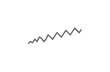
\begin{tikzpicture}[x=0.08em, y=0.08em, line width=0.4pt]
                \draw[FooterGray] (0,3) -- (1,4) -- (2,3.5) -- (3,5) -- (4,4) -- (5,6) -- (6,5.5) -- (7,4) -- (8,5) -- (9,7) -- (10,6) -- (11,5) -- (12,6.5) -- (13,8) -- (14,7) -- (15,6) -- (16,7.5) -- (17,9) -- (18,8) -- (19,7) -- (20,8.5) -- (21,10) -- (22,9) -- (23,8) -- (24,9.5);
            \end{tikzpicture}%
        }%
        \hskip0.5cm%
    }%
    \vskip6pt%
}

%=============================================================================
% PACHETE
%=============================================================================
\usepackage[utf8]{inputenc}
\usepackage[T1]{fontenc}
\usepackage[romanian]{babel}
\usepackage{amsmath, amssymb, amsthm}
\usepackage{mathtools}
\usepackage{bm}
\usepackage{tikz}
\usetikzlibrary{arrows.meta, positioning, shapes, calc, decorations.pathreplacing, shadings}
\usepackage{booktabs}
\usepackage{multirow}
\usepackage{array}
\usepackage{graphicx}
\usepackage{hyperref}
\usepackage{colortbl}
\hypersetup{colorlinks=true, linkcolor=MainBlue, urlcolor=MainBlue}
\graphicspath{{../../logos/}{../../charts/}}
\hfuzz=2pt  % Suppress tiny overfull warnings (<2pt)
\vfuzz=2pt  % Suppress tiny vertical overfull warnings (<2pt)

%=============================================================================
% COMANDA QUANTLET
%=============================================================================
\newcommand{\quantlet}[2]{%
    \hfill\href{#2}{%
        \raisebox{-0.15em}{\includegraphics[height=0.7em]{ql_logo.png}}%
        \textcolor{MainBlue}{\tiny\ #1}%
    }%
}

%=============================================================================
% CENTRED MINIPAGE (fara spatiu vertical suplimentar)
%=============================================================================
\newenvironment{cminipage}[1]{%
    \par\noindent\hfill\begin{minipage}{#1}\ignorespaces
}{%
    \end{minipage}\hfill\null\par
}

%=============================================================================
% COMENZI PERSONALIZATE
%=============================================================================
\newcommand{\E}{\mathbb{E}}
\newcommand{\Var}{\text{Var}}
\newcommand{\Cov}{\text{Cov}}
\newcommand{\Corr}{\text{Corr}}
\newcommand{\R}{\mathbb{R}}
\newcommand{\RMSE}{\text{RMSE}}
\newcommand{\MAE}{\text{MAE}}
\newcommand{\MAPE}{\text{MAPE}}

\newcommand{\correct}{\textcolor{Forest}{\checkmark}}
\newcommand{\incorrect}{\textcolor{Crimson}{\texttimes}}

%=============================================================================
% PAGINA TITLU PERSONALIZATA
%=============================================================================
\defbeamertemplate*{title page}{hybrid}[1][]
{
    \vspace{0.2cm}
    \begin{center}
        \href{https://www.ase.ro}{\includegraphics[height=1.0cm]{ase_logo.png}}\hspace{0.3cm}%
        \href{https://theida.net}{\includegraphics[height=1.0cm]{ida_logo.png}}\hspace{0.3cm}%
        \href{https://blockchain-research-center.com}{\includegraphics[height=1.0cm]{brc_logo.png}}\hspace{0.3cm}%
        \href{https://www.ai4efin.ase.ro}{\includegraphics[height=1.0cm]{ai4efin_logo.png}}\hspace{0.3cm}%
        \href{https://ipe.ro/new}{\includegraphics[height=1.0cm]{acad_logo.png}}\hspace{0.3cm}%
        \href{https://www.digital-finance-msca.com}{\includegraphics[height=1.0cm]{msca_logo.png}}%
    \end{center}

    \vspace{0.6cm}

    \begin{center}
        \begin{minipage}{0.1\textwidth}
            \centering
            \href{https://quantlet.com}{\includegraphics[height=1.1cm]{ql_logo.png}}
        \end{minipage}%
        \begin{minipage}{0.78\textwidth}
            \centering
            {\LARGE\bfseries\usebeamercolor[fg]{title}\inserttitle}

            \vspace{0.3cm}

            {\usebeamerfont{subtitle}\usebeamercolor[fg]{title}\insertsubtitle}
        \end{minipage}%
        \begin{minipage}{0.1\textwidth}
            \centering
            \href{https://quantinar.com}{\includegraphics[height=1.1cm]{qr_logo.png}}
        \end{minipage}
    \end{center}

    \vspace{0.6cm}

    \hspace{0.5cm}{\usebeamerfont{author}\insertauthor}

    \vspace{0.3cm}

    \hspace{0.5cm}\begin{minipage}[t]{0.9\textwidth}
        \raggedright\small\insertinstitute
    \end{minipage}
}

%=============================================================================
% INFORMATII TITLU
%=============================================================================
\title[Analiza Seriilor de Timp]{Analiza și Prognoza seriilor de timp}
\subtitle{Seminar 8: Extensii moderne}
\author[D.T. Pele]{Daniel Traian PELE}
\institute{Academia de Studii Economice din București\\
IDA Institute Digital Assets\\
Blockchain Research Center\\
AI4EFin Artificial Intelligence for Energy Finance\\
Academia Română, Institutul de Prognoză Economică\\
MSCA Digital Finance}
\date{}

\begin{document}

% Title page (no header/footer)
{
\setbeamertemplate{headline}{}
\setbeamertemplate{footline}{}
\begin{frame}
    \titlepage
\end{frame}
}

%=============================================================================
% OUTLINE
%=============================================================================
\begin{frame}{Cuprins Seminar}
    \begin{cminipage}{0.95\textwidth}
    \textbf{\large Structura seminarului:}

    \vspace{0.4cm}

    \begin{enumerate}
        \item[\textcolor{MainBlue}{\textbf{1.}}] \textbf{Test de Recapitulare} -- Verificarea cunoștințelor
        \vspace{0.15cm}
        \item[\textcolor{MainBlue}{\textbf{2.}}] \textbf{Întrebări Adevărat/Fals} -- Verificări conceptuale
        \vspace{0.15cm}
        \item[\textcolor{MainBlue}{\textbf{3.}}] \textbf{Probleme Practice} -- Practică aplicată
        \vspace{0.15cm}
        \item[\textcolor{MainBlue}{\textbf{4.}}] \textbf{Rezumat} -- Sinteză finală
        \vspace{0.15cm}
        \item[\textcolor{MainBlue}{\textbf{5.}}] \textbf{Exerciții cu asistență AI} -- Inteligență artificială aplicată
    \end{enumerate}
    \end{cminipage}
\end{frame}

%=============================================================================
% TEST DE RECAPITULARE
%=============================================================================
\section{Test de Recapitulare}

\begin{frame}{Test 1: Exponentul Hurst}
    \begin{alertblock}{Întrebare}
        O serie de timp are exponentul Hurst $H = 0.8$. Ce ne indică acest lucru?
    \end{alertblock}

    \vspace{0.3cm}

    \begin{block}{Variante de răspuns}
        \textcolor{MainBlue}{\textbf{(A)}} Seria este un mers aleator pur\\[3pt]
        \textcolor{MainBlue}{\textbf{(B)}} Seria are memorie lungă și este persistentă (trend-following)\\[3pt]
        \textcolor{MainBlue}{\textbf{(C)}} Seria este anti-persistentă (mean-reverting)\\[3pt]
        \textcolor{MainBlue}{\textbf{(D)}} Seria este staționară I(0)
    \end{block}

    \vspace{0.5cm}
    \begin{flushright}\textit{Răspunsul pe slide-ul următor...}\end{flushright}
\end{frame}

\begin{frame}{Test 1: Răspuns}
    \begin{exampleblock}{Răspuns: B -- Memorie lungă și persistență}
        \textbf{Interpretare Exponent Hurst:}
        \begin{itemize}
            \item $H = 0.5$: Mers aleator (fără memorie)
            \item $0.5 < H < 1$: \textbf{Persistență} -- tendința continuă
            \item $0 < H < 0.5$: Anti-persistență -- revenire la medie
        \end{itemize}

        \vspace{0.3cm}
        Cu $H = 0.8 > 0.5$:
        \begin{itemize}
            \item Seria are \textbf{memorie lungă}
            \item Valorile mari tind să fie urmate de valori mari
            \item Autocorrelațiile descresc lent (hiperbolic, nu exponențial)
        \end{itemize}
    \end{exampleblock}
    \quantlet{TSA\_ch8\_hurst}{https://github.com/QuantLet/TSA/tree/main/TSA_ch8/TSA_ch8_hurst}
\end{frame}

\begin{frame}{Test 2: Parametrul de Diferențiere Fracționară}
    \begin{alertblock}{Întrebare}
        În modelul ARFIMA(p, d, q), parametrul $d$ poate lua valori:
    \end{alertblock}

    \vspace{0.3cm}

    \begin{block}{Variante de răspuns}
        \textcolor{MainBlue}{\textbf{(A)}} Doar valori întregi (0, 1, 2, ...)\\[3pt]
        \textcolor{MainBlue}{\textbf{(B)}} Doar $d = 0$ sau $d = 1$\\[3pt]
        \textcolor{MainBlue}{\textbf{(C)}} Orice valoare reală, inclusiv fracționară\\[3pt]
        \textcolor{MainBlue}{\textbf{(D)}} Doar valori negative
    \end{block}

    \vspace{0.5cm}
    \begin{flushright}\textit{Răspunsul pe slide-ul următor...}\end{flushright}
\end{frame}

\begin{frame}{Test 2: Răspuns}
    \begin{exampleblock}{Răspuns: C -- Orice valoare reală}
        \textbf{Diferențiere fracționară}: $(1-L)^d$ cu $d \in \mathbb{R}$

        \vspace{0.3cm}
        \textbf{Interpretare valori $d$:}
        \begin{itemize}
            \item $d = 0$: Seria staționară (ARMA)
            \item $0 < d < 0.5$: Memorie lungă, staționară
            \item $d = 0.5$: Granița staționar/nestaționară
            \item $0.5 < d < 1$: Memorie lungă, nestaționară
            \item $d = 1$: Diferențiere completă (ARIMA clasic)
        \end{itemize}

        \vspace{0.2cm}
        \textbf{Relația cu Hurst}: $d = H - 0.5$
    \end{exampleblock}
    \quantlet{TSA\_ch8\_arfima}{https://github.com/QuantLet/TSA/tree/main/TSA_ch8/TSA_ch8_arfima}
\end{frame}

\begin{frame}{Test 3: Memoria Lungă în Serii Financiare}
    \begin{alertblock}{Întrebare}
        În ce serie financiară este memoria lungă cel mai frecvent documentată?
    \end{alertblock}

    \vspace{0.3cm}

    \begin{block}{Variante de răspuns}
        \textcolor{MainBlue}{\textbf{(A)}} Prețurile acțiunilor\\[3pt]
        \textcolor{MainBlue}{\textbf{(B)}} Randamentele zilnice\\[3pt]
        \textcolor{MainBlue}{\textbf{(C)}} Volatilitatea (pătratul randamentelor)\\[3pt]
        \textcolor{MainBlue}{\textbf{(D)}} Volumul de tranzacționare
    \end{block}

    \vspace{0.5cm}
    \begin{flushright}\textit{Răspunsul pe slide-ul următor...}\end{flushright}
\end{frame}

\begin{frame}{Test 3: Răspuns}
    \begin{exampleblock}{Răspuns: C -- Volatilitatea}
        \textbf{Fapte stilizate din finanțe:}
        \begin{itemize}
            \item \textbf{Randamentele}: Aproximativ fără memorie ($H \approx 0.5$)
            \item \textbf{Volatilitatea}: Memorie lungă pronunțată ($H \approx 0.7-0.9$)
        \end{itemize}

        \vspace{0.3cm}
        \textbf{De ce?}
        \begin{itemize}
            \item Volatility clustering: perioade agitate urmate de perioade agitate
            \item Persistența șocurilor în varianță
            \item FIGARCH: modelează explicit memoria lungă în volatilitate
        \end{itemize}

        \vspace{0.2cm}
        {\footnotesize Acest fapt stilizat este baza modelelor FIGARCH și HAR-RV.}
    \end{exampleblock}
    \quantlet{TSA\_ch8\_long\_memory}{https://github.com/QuantLet/TSA/tree/main/TSA_ch8/TSA_ch8_long_memory}
\end{frame}

\begin{frame}{Test 4: Feature Engineering}
    \begin{alertblock}{Întrebare}
        Pentru a aplica Random Forest pe serii de timp, trebuie să creăm:
    \end{alertblock}

    \vspace{0.3cm}

    \begin{block}{Variante de răspuns}
        \textcolor{MainBlue}{\textbf{(A)}} Variabile dummy pentru fiecare observație\\[3pt]
        \textcolor{MainBlue}{\textbf{(B)}} Caracteristici lag și statistici rolling\\[3pt]
        \textcolor{MainBlue}{\textbf{(C)}} Transformări Fourier ale seriei\\[3pt]
        \textcolor{MainBlue}{\textbf{(D)}} Numai prima diferență a seriei
    \end{block}

    \vspace{0.5cm}
    \begin{flushright}\textit{Răspunsul pe slide-ul următor...}\end{flushright}
\end{frame}

\begin{frame}{Test 4: Răspuns}
    \begin{exampleblock}{Răspuns: B -- Caracteristici lag și statistici rolling}
        \textbf{Feature Engineering pentru Serii de timp:}

        \vspace{0.2cm}
        \begin{itemize}
            \item \textbf{Lag features}: $y_{t-1}, y_{t-2}, \ldots, y_{t-k}$
            \item \textbf{Rolling statistics}:
                \begin{itemize}
                    \item Media mobilă: $\bar{y}_{t,w}$
                    \item Deviația standard mobilă: $\sigma_{t,w}$
                    \item Min/Max pe fereastră
                \end{itemize}
            \item \textbf{Caracteristici calendaristice}: ziua săptămânii, luna, etc.
        \end{itemize}

        \vspace{0.2cm}
        \textbf{Important}: Transformă problema de prognoză în problemă de regresie supervizată!
    \end{exampleblock}
    \quantlet{TSA\_ch8\_ml\_forecast}{https://github.com/QuantLet/TSA/tree/main/TSA_ch8/TSA_ch8_ml_forecast}
\end{frame}

\begin{frame}{Test 5: Validarea încrucișată pentru Serii de timp}
    \begin{alertblock}{Întrebare}
        De ce NU putem folosi k-fold cross-validation standard pentru serii de timp?
    \end{alertblock}

    \vspace{0.3cm}

    \begin{block}{Variante de răspuns}
        \textcolor{MainBlue}{\textbf{(A)}} Este prea lent pentru serii lungi\\[3pt]
        \textcolor{MainBlue}{\textbf{(B)}} Încalcă ordinea temporală și cauzează data leakage\\[3pt]
        \textcolor{MainBlue}{\textbf{(C)}} Funcționează doar pentru clasificare\\[3pt]
        \textcolor{MainBlue}{\textbf{(D)}} Necesită prea multe date
    \end{block}

    \vspace{0.5cm}
    \begin{flushright}\textit{Răspunsul pe slide-ul următor...}\end{flushright}
\end{frame}

\begin{frame}{Test 5: Răspuns}
    \begin{exampleblock}{Răspuns: B -- Încalcă ordinea temporală}
        \textbf{Problema cu k-fold standard:}
        \begin{itemize}
            \item Amestecă observațiile temporal
            \item Antrenează pe date din viitor, testează pe trecut
            \item \textbf{Data leakage} $\Rightarrow$ performanță supraestimată
        \end{itemize}

        \vspace{0.3cm}
        \textbf{Soluția: Time Series Split (Walk-Forward)}
        \begin{center}
        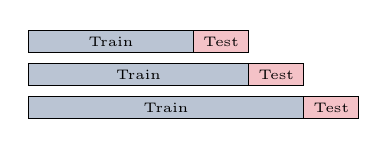
\begin{tikzpicture}[scale=0.7]
            \draw[fill=MainBlue!30] (0,0) rectangle (3,0.4) node[midway] {\tiny Train};
            \draw[fill=Crimson!30] (3,0) rectangle (4,0.4) node[midway] {\tiny Test};
            \draw[fill=MainBlue!30] (0,-0.6) rectangle (4,-0.2) node[midway] {\tiny Train};
            \draw[fill=Crimson!30] (4,-0.6) rectangle (5,-0.2) node[midway] {\tiny Test};
            \draw[fill=MainBlue!30] (0,-1.2) rectangle (5,-0.8) node[midway] {\tiny Train};
            \draw[fill=Crimson!30] (5,-1.2) rectangle (6,-0.8) node[midway] {\tiny Test};
        \end{tikzpicture}
        \end{center}
    \end{exampleblock}
    \quantlet{TSA\_ch8\_cross\_validation}{https://github.com/QuantLet/TSA/tree/main/TSA_ch8/TSA_ch8_cross_validation}
\end{frame}

\begin{frame}{Test 6: Importanța Variabilelor în Random Forest}
    \begin{alertblock}{Întrebare}
        Importanța variabilelor în Random Forest pentru serii de timp ne ajută să:
    \end{alertblock}

    \vspace{0.3cm}

    \begin{block}{Variante de răspuns}
        \textcolor{MainBlue}{\textbf{(A)}} Să eliminăm toate variabilele cu importanță mică\\[3pt]
        \textcolor{MainBlue}{\textbf{(B)}} Să identificăm care lag-uri și caracteristici sunt cele mai predictive\\[3pt]
        \textcolor{MainBlue}{\textbf{(C)}} Să determinăm cauzalitatea Granger\\[3pt]
        \textcolor{MainBlue}{\textbf{(D)}} Să calculăm intervalele de încredere
    \end{block}

    \vspace{0.5cm}
    \begin{flushright}\textit{Răspunsul pe slide-ul următor...}\end{flushright}
\end{frame}

\begin{frame}{Test 6: Răspuns}
    \begin{exampleblock}{Răspuns: B -- Identifică caracteristicile predictive}
        \textbf{Utilizări ale importanței variabilelor:}
        \begin{itemize}
            \item Înțelegerea structurii temporale
            \item Selectarea numărului optim de lag-uri
            \item Identificarea factorilor relevanți
        \end{itemize}

        \vspace{0.3cm}
        \textbf{Atenție:}
        \begin{itemize}
            \item Importanța NU implică cauzalitate
            \item Variabilele corelate pot împărtăși importanța
            \item Folosiți pentru interpretare, nu pentru inferență cauzală
        \end{itemize}
    \end{exampleblock}
    \quantlet{TSA\_ch8\_feature\_importance}{https://github.com/QuantLet/TSA/tree/main/TSA_ch8/TSA_ch8_feature_importance}
\end{frame}

\begin{frame}{Test 7: Avantajul LSTM}
    \begin{alertblock}{Întrebare}
        Care este principalul avantaj al LSTM față de RNN simple?
    \end{alertblock}

    \vspace{0.3cm}

    \begin{block}{Variante de răspuns}
        \textcolor{MainBlue}{\textbf{(A)}} Este mai rapidă la antrenare\\[3pt]
        \textcolor{MainBlue}{\textbf{(B)}} Rezolvă problema gradienților care dispar/explodează\\[3pt]
        \textcolor{MainBlue}{\textbf{(C)}} Necesită mai puține date\\[3pt]
        \textcolor{MainBlue}{\textbf{(D)}} Este mai ușor de interpretat
    \end{block}

    \vspace{0.5cm}
    \begin{flushright}\textit{Răspunsul pe slide-ul următor...}\end{flushright}
\end{frame}

\begin{frame}{Test 7: Răspuns}
    \begin{exampleblock}{Răspuns: B -- Rezolvă problema gradienților}
        \textbf{Problema RNN Simple:}
        \begin{itemize}
            \item Gradienții scad exponențial cu lungimea secvenței
            \item Nu pot învăța dependențe pe termen lung
        \end{itemize}

        \vspace{0.3cm}
        \textbf{Soluția LSTM:}
        \begin{itemize}
            \item \textbf{Cell state}: Autostradă pentru flux de informație
            \item \textbf{Forget gate}: Decide ce să uite
            \item \textbf{Input gate}: Decide ce să rețină
            \item \textbf{Output gate}: Decide ce să producă
        \end{itemize}

        \vspace{0.2cm}
        Gradienții pot „curge" prin cell state fără degradare!
    \end{exampleblock}
    \quantlet{TSA\_ch8\_lstm}{https://github.com/QuantLet/TSA/tree/main/TSA_ch8/TSA_ch8_lstm}
\end{frame}

\begin{frame}{Test 8: Pregătirea Datelor pentru LSTM}
    \begin{alertblock}{Întrebare}
        Înainte de antrenarea LSTM, datele trebuie:
    \end{alertblock}

    \vspace{0.3cm}

    \begin{block}{Variante de răspuns}
        \textcolor{MainBlue}{\textbf{(A)}} Transformate logaritmic\\[3pt]
        \textcolor{MainBlue}{\textbf{(B)}} Normalizate/standardizate la intervalul [0,1] sau [-1,1]\\[3pt]
        \textcolor{MainBlue}{\textbf{(C)}} Diferențiate de ordinul 2\\[3pt]
        \textcolor{MainBlue}{\textbf{(D)}} Convertite la numere întregi
    \end{block}

    \vspace{0.5cm}
    \begin{flushright}\textit{Răspunsul pe slide-ul următor...}\end{flushright}
\end{frame}

\begin{frame}{Test 8: Răspuns}
    \begin{exampleblock}{Răspuns: B -- Normalizate/standardizate}
        \textbf{De ce normalizare?}
        \begin{itemize}
            \item Funcțiile de activare (sigmoid, tanh) funcționează în intervale limitate
            \item Convergență mai rapidă
            \item Stabilitate numerică
        \end{itemize}

        \vspace{0.3cm}
        \textbf{Metode comune:}
        \begin{itemize}
            \item \textbf{Min-Max}: $x' = \frac{x - x_{min}}{x_{max} - x_{min}}$ $\succ$ [0, 1]
            \item \textbf{Standard}: $x' = \frac{x - \mu}{\sigma}$ $\succ$ media 0, std 1
        \end{itemize}

        \vspace{0.2cm}
        \textbf{Important}: Fit pe train, transform pe train+test!
    \end{exampleblock}
    \quantlet{TSA\_ch8\_lstm\_preprocessing}{https://github.com/QuantLet/TSA/tree/main/TSA_ch8/TSA_ch8_lstm_preprocessing}
\end{frame}

\begin{frame}{Test 9: Hiperparametri LSTM}
    \begin{alertblock}{Întrebare}
        Care NU este un hiperparametru tipic pentru LSTM?
    \end{alertblock}

    \vspace{0.3cm}

    \begin{block}{Variante de răspuns}
        \textcolor{MainBlue}{\textbf{(A)}} Numărul de unități (neuroni) pe strat\\[3pt]
        \textcolor{MainBlue}{\textbf{(B)}} Lungimea secvenței de intrare\\[3pt]
        \textcolor{MainBlue}{\textbf{(C)}} Learning rate\\[3pt]
        \textcolor{MainBlue}{\textbf{(D)}} Parametrul de diferențiere $d$
    \end{block}

    \vspace{0.5cm}
    \begin{flushright}\textit{Răspunsul pe slide-ul următor...}\end{flushright}
\end{frame}

\begin{frame}{Test 9: Răspuns}
    \begin{exampleblock}{Răspuns: D -- Parametrul $d$}
        $d$ este specific modelelor ARFIMA, nu LSTM!

        \vspace{0.3cm}
        \textbf{Hiperparametri LSTM:}
        \begin{itemize}
            \item \textbf{Arhitectură}: nr. straturi, unități/strat
            \item \textbf{Secvență}: lungime lookback
            \item \textbf{Training}: learning rate, batch size, epochs
            \item \textbf{Regularizare}: dropout, early stopping
        \end{itemize}

        \vspace{0.2cm}
        \textbf{Tuning}: Grid search sau Bayesian optimization cu time series CV
    \end{exampleblock}
    \quantlet{TSA\_ch8\_lstm\_tuning}{https://github.com/QuantLet/TSA/tree/main/TSA_ch8/TSA_ch8_lstm_tuning}
\end{frame}

%=============================================================================
% ÎNTREBĂRI ADEVĂRAT/FALS
%=============================================================================
\section{Întrebări Adevărat/Fals}

\begin{frame}{Adevărat sau Fals? --- Întrebări}
    \begin{cminipage}{0.95\textwidth}
    \footnotesize
    \begin{center}
    \begin{tabular}{p{9cm}c}
        \toprule
        \textbf{Afirmație} & \textbf{A/F?} \\
        \midrule
        1. Modelele ARFIMA pot captura dependență pe termen lung. & ? \\[0.15cm]
        2. Parametrul $d$ în ARFIMA trebuie să fie un număr întreg. & ? \\[0.15cm]
        3. Rețelele LSTM sunt mai bune decât ARIMA în toate situațiile. & ? \\[0.15cm]
        4. Random Forest necesită caracteristici (features) create manual. & ? \\[0.15cm]
        5. Validarea încrucișată standard (k-fold) este potrivită pentru serii de timp. & ? \\[0.15cm]
        6. Exponentul Hurst $H > 0.5$ indică memorie lungă pozitivă. & ? \\
        \bottomrule
    \end{tabular}
    \end{center}
    \end{cminipage}
\end{frame}

\begin{frame}{Adevărat sau Fals? --- Răspunsuri}
    \begin{cminipage}{0.95\textwidth}
    \scriptsize
    \begin{center}
    \begin{tabular}{p{7.5cm}cc}
        \toprule
        \textbf{Afirmație} & \textbf{A/F} & \textbf{Explicație} \\
        \midrule
        1. ARFIMA captează dependență pe termen lung. & \textcolor{Forest}{\textbf{A}} & {\tiny $d$ fracționar} \\[0.08cm]
        2. $d$ în ARFIMA trebuie să fie întreg. & \textcolor{Crimson}{\textbf{F}} & {\tiny $d \in (0, 0.5)$ fracționar} \\[0.08cm]
        3. LSTM mai bun decât ARIMA mereu. & \textcolor{Crimson}{\textbf{F}} & {\tiny Depinde de date și eșantion} \\[0.08cm]
        4. RF necesită features manuale. & \textcolor{Forest}{\textbf{A}} & {\tiny Lag-uri, calendar, etc.} \\[0.08cm]
        5. k-fold CV potrivit pt serii de timp. & \textcolor{Crimson}{\textbf{F}} & {\tiny Încalcă ordonarea temporală} \\[0.08cm]
        6. $H > 0.5$ indică memorie lungă pozitivă. & \textcolor{Forest}{\textbf{A}} & {\tiny $H = 0.5$: fără memorie} \\
        \bottomrule
    \end{tabular}
    \end{center}
    \end{cminipage}
\end{frame}

%=============================================================================
% PROBLEME PRACTICE
%=============================================================================
\section{Probleme Practice}

\begin{frame}{Problemă 1: Estimarea Exponentului Hurst}
    \begin{block}{Enunț}
        Fie seria zilnică de randamente Bitcoin. Estimați exponentul Hurst folosind metoda R/S și interpretați rezultatul.
    \end{block}

    \vspace{0.3cm}
    \textbf{Pași de rezolvare:}
    \begin{enumerate}
        \item Calculați media pe subintervale de diferite lungimi $n$
        \item Pentru fiecare $n$: calculați Range($R$) și Std($S$)
        \item Raportul $R/S$ crește ca $n^H$
        \item Fit regresie: $\log(R/S) = H \cdot \log(n) + c$
    \end{enumerate}

    \vspace{0.2cm}
    \textbf{Cod Python}: \texttt{nolds.hurst\_rs(returns)}
\end{frame}

\begin{frame}{Problemă 1: Soluție și Interpretare}
    \begin{exampleblock}{Rezultat Tipic pentru Bitcoin}
        \begin{itemize}
            \item Randamente: $H \approx 0.45-0.55$ (aproape mers aleator)
            \item Volatilitate (|returns|): $H \approx 0.75-0.85$ (memorie lungă!)
        \end{itemize}
    \end{exampleblock}

    \vspace{0.3cm}
    \textbf{Interpretare:}
    \begin{itemize}
        \item Randamentele sunt greu de prognozat (EMH aproximativ validă)
        \item Volatilitatea este predictibilă pe termen lung
        \item Implicații pentru managementul riscului și VaR
    \end{itemize}

    \vspace{0.2cm}
    \textbf{Aplicație}: Modelele FIGARCH pot fi superioare GARCH standard
    \quantlet{TSA\_ch8\_hurst}{https://github.com/QuantLet/TSA/tree/main/TSA_ch8/TSA_ch8_hurst}
\end{frame}

\begin{frame}{Problemă 2: Random Forest pentru Prognoză}
    \begin{block}{Enunț}
        Construiți un model Random Forest pentru prognoza prețului Bitcoin la orizontul de 1 zi. Evaluați folosind TimeSeriesSplit.
    \end{block}

    \vspace{0.3cm}
    \textbf{Pipeline:}
    \begin{enumerate}
        \item \textbf{Feature engineering}:
            \begin{itemize}
                \item Lag-uri: $y_{t-1}, y_{t-2}, \ldots, y_{t-7}$
                \item Rolling mean/std: 7, 14, 30 zile
            \end{itemize}
        \item \textbf{Train/Test split}: TimeSeriesSplit(n\_splits=5)
        \item \textbf{Model}: RandomForestRegressor(n\_estimators=100)
        \item \textbf{Evaluare}: RMSE, MAE, Direction Accuracy
    \end{enumerate}
\end{frame}

\begin{frame}{Problemă 2: Cod și Rezultate}
    \begin{exampleblock}{Cod Python}
        {\footnotesize
        \texttt{from sklearn.ensemble import RandomForestRegressor}\\
        \texttt{from sklearn.model\_selection import TimeSeriesSplit}\\[0.2cm]
        \texttt{tscv = TimeSeriesSplit(n\_splits=5)}\\
        \texttt{rf = RandomForestRegressor(n\_estimators=100)}\\[0.2cm]
        \texttt{for train\_idx, test\_idx in tscv.split(X):}\\
        \texttt{~~~~rf.fit(X[train\_idx], y[train\_idx])}\\
        \texttt{~~~~pred = rf.predict(X[test\_idx])}
        }
    \end{exampleblock}

    \vspace{0.2cm}
    \textbf{Rezultate tipice}:
    \begin{itemize}
        \item Direction accuracy: 52-55\% (puțin peste random)
        \item Feature importance: lag-1 și rolling\_std domină
    \end{itemize}
    \quantlet{TSA\_ch8\_random\_forest}{https://github.com/QuantLet/TSA/tree/main/TSA_ch8/TSA_ch8_random_forest}
\end{frame}

\begin{frame}{Problemă 3: LSTM pentru Serii de timp}
    \begin{block}{Enunț}
        Implementați un model LSTM simplu pentru prognoza Bitcoin. Comparați cu Random Forest.
    \end{block}

    \vspace{0.3cm}
    \textbf{Arhitectură LSTM simplă:}
    \begin{enumerate}
        \item Input: secvențe de 30 de zile
        \item LSTM layer: 50 unități
        \item Dense output: 1 neuron (prognoza)
        \item Loss: MSE, Optimizer: Adam
    \end{enumerate}

    \vspace{0.2cm}
    \textbf{Pași importanți}:
    \begin{itemize}
        \item Normalizare MinMaxScaler
        \item Reshape la [samples, timesteps, features]
        \item Early stopping pentru a evita supraajustare
    \end{itemize}
\end{frame}

\begin{frame}{Problemă 3: Cod LSTM}
    \begin{exampleblock}{Cod Keras/TensorFlow}
        {\footnotesize
        \texttt{from tensorflow.keras.models import Sequential}\\
        \texttt{from tensorflow.keras.layers import LSTM, Dense}\\[0.2cm]
        \texttt{model = Sequential([}\\
        \texttt{~~~~LSTM(50, input\_shape=(30, 1)),}\\
        \texttt{~~~~Dense(1)}\\
        \texttt{])}\\[0.2cm]
        \texttt{model.compile(optimizer='adam', loss='mse')}\\
        \texttt{model.fit(X\_train, y\_train, epochs=50,}\\
        \texttt{~~~~~~~~~~validation\_split=0.1, verbose=0)}
        }
    \end{exampleblock}

    \vspace{0.2cm}
    \textbf{Comparație tipică RF vs LSTM}:
    \begin{itemize}
        \item RMSE similar (LSTM ușor mai bun pe date netede)
        \item RF: mai rapid, mai interpretabil
        \item LSTM: captează mai bine pattern-uri complexe
    \end{itemize}
    \quantlet{TSA\_ch8\_lstm}{https://github.com/QuantLet/TSA/tree/main/TSA_ch8/TSA_ch8_lstm}
\end{frame}

%=============================================================================
% REZUMAT
%=============================================================================
\section{Rezumat}

\begin{frame}{Rezumat: Când să folosim Fiecare Metodă}
    \vspace{-0.9cm}
    \begin{block}{ARFIMA}
        \begin{itemize}
            \item Serii cu memorie lungă (volatilitate, hidrologie)
            \item Când $0 < d < 0.5$ este teoretic justificat
            \item Interpretabilitate statistică importantă
        \end{itemize}
    \end{block}

    \begin{block}{Random Forest}
        \begin{itemize}
            \item Relații neliniare între caracteristici
            \item Feature importance pentru înțelegere
            \item Date structurate, nu foarte lungi
        \end{itemize}
    \end{block}

    \begin{block}{LSTM}
        \begin{itemize}
            \item Secvențe lungi cu dependențe complexe
            \item Date suficiente pentru deep learning
            \item Pattern-uri dificil de capturat cu metode clasice
        \end{itemize}
    \end{block}
\end{frame}

\begin{frame}[shrink=5]{Formule cheie}
    \vspace{-0.8cm}
    \begin{block}{ARFIMA și Memorie Lungă}
        \begin{itemize}
            \item Diferențiere fracționară: $(1-L)^d y_t = \varepsilon_t$
            \item Exponent Hurst: $d = H - 0.5$
            \item ACF pentru memorie lungă: $\rho(k) \sim k^{2d-1}$ (descreștere lentă)
        \end{itemize}
    \end{block}

    \begin{block}{Machine Learning}
        \begin{itemize}
            \item Feature lag: $X_t = [y_{t-1}, y_{t-2}, \ldots, y_{t-k}]$
            \item RMSE: $\sqrt{\frac{1}{n}\sum(y_i - \hat{y}_i)^2}$
            \item Direction Accuracy: $\frac{1}{n}\sum \mathbf{1}[\text{sign}(\Delta y) = \text{sign}(\Delta \hat{y})]$
        \end{itemize}
    \end{block}

    \begin{block}{LSTM}
        \begin{itemize}
            \item Forget gate: $f_t = \sigma(W_f \cdot [h_{t-1}, x_t] + b_f)$
            \item Cell update: $C_t = f_t * C_{t-1} + i_t * \tilde{C}_t$
        \end{itemize}
    \end{block}
\end{frame}

%=============================================================================
% EXERCIȚII CU ASISTENȚĂ AI
%=============================================================================
\section{Exerciții cu asistență AI}

\begin{frame}{Exercițiu AI: Gândire critică}
    \begin{cminipage}{0.95\textwidth}
    \vspace{-0.3cm}
    \begin{block}{\footnotesize Prompt de testat în ChatGPT / Claude / Copilot}
        {\footnotesize
        ``Compară performanța de prognoză a unui model ARIMA, Random Forest și LSTM pe datele de consum de electricitate. Care model este cel mai bun?''
        }
    \end{block}
    \vspace{-2mm}
    {\footnotesize
    \textbf{Exercițiu}:
    \begin{enumerate}\setlength{\itemsep}{0pt}
        \item Rulați prompt-ul într-un LLM la alegere și analizați critic răspunsul.
        \item AI folosește aceeași împărțire train/test pentru toate modelele?
        \item Hiperparametrii LSTM (număr de neuroni, epoci, learning rate) sunt optimizați sau impliciți?
        \item Feature engineering-ul pentru Random Forest include lag-uri, variabile calendar?
        \item Comparația este pe baza RMSE out-of-sample sau in-sample?
    \end{enumerate}
    }
    \vspace{-2mm}
    \begin{alertblock}{}
        {\footnotesize \textbf{Atenție}: Codul generat de AI poate rula fără erori și arăta profesional. \textit{Asta nu înseamnă că e corect.}}
    \end{alertblock}
    \end{cminipage}
\end{frame}

%=============================================================================
% THANK YOU SLIDE
%=============================================================================
\begin{frame}{}
    \begin{cminipage}{0.95\textwidth}
    \centering
    \Huge\textcolor{IDAred}{Vă mulțumim!}

    \vspace{1cm}

    \Large\textcolor{MainBlue}{Întrebări?}

    \vspace{0.8cm}

    \normalsize
    Materialele seminarului sunt disponibile la: \url{https://danpele.github.io/Time-Series-Analysis/}

    \vspace{0.2cm}

    \href{https://quantlet.com}{\raisebox{-0.15em}{\includegraphics[height=0.8em]{ql_logo.png}} Quantlet} \hspace{0.5cm}
    \href{https://quantinar.com}{\raisebox{-0.15em}{\includegraphics[height=0.8em]{qr_logo.png}} Quantinar}
    \end{cminipage}
\end{frame}

%=============================================================================
% BIBLIOGRAFIE
%=============================================================================
\begin{frame}{Bibliografie I}
    \begin{block}{Manuale fundamentale}
        {\small
        \begin{itemize}
            \item Hyndman, R.J., \& Athanasopoulos, G. (2021). \textit{Forecasting: Principles and Practice}, 3rd ed., OTexts.
            \item Shumway, R.H., \& Stoffer, D.S. (2017). \textit{Time Series Analysis and Its Applications}, 4th ed., Springer.
            \item Brockwell, P.J., \& Davis, R.A. (2016). \textit{Introduction to Time Series and Forecasting}, 3rd ed., Springer.
        \end{itemize}
        }
    \end{block}

    \begin{exampleblock}{Serii de timp financiare}
        {\small
        \begin{itemize}
            \item Tsay, R.S. (2010). \textit{Analysis of Financial Time Series}, 3rd ed., Wiley.
            \item Franke, J., Härdle, W.K., \& Hafner, C.M. (2019). \textit{Statistics of Financial Markets}, 4th ed., Springer.
        \end{itemize}
        }
    \end{exampleblock}
\end{frame}

\begin{frame}{Bibliografie II}
    \begin{block}{Abordari moderne si Machine Learning}
        {\small
        \begin{itemize}
            \item Nielsen, A. (2019). \textit{Practical Time Series Analysis}, O'Reilly Media.
            \item Petropoulos, F., et al. (2022). \textit{Forecasting: Theory and Practice}, International Journal of Forecasting.
            \item Makridakis, S., Spiliotis, E., \& Assimakopoulos, V. (2020). The M4 Competition, International Journal of Forecasting.
        \end{itemize}
        }
    \end{block}

    \begin{exampleblock}{Resurse online si cod}
        {\small
        \begin{itemize}
            \item \textbf{Quantlet}: \url{https://quantlet.com} --- Repository de cod pentru statistica
            \item \textbf{Quantinar}: \url{https://quantinar.com} --- Platforma de invatare metode cantitative
            \item \textbf{GitHub TSA}: \url{https://github.com/QuantLet/TSA} --- Cod Python pentru fiecare capitol
        \end{itemize}
        }
    \end{exampleblock}
\end{frame}

\end{document}